% LaTeX formatting example for NERCCS
% Revised on 8/23/2018 by Hiroki Sayama

\documentclass[12pt]{article}
\usepackage[letterpaper,margin=1in]{geometry}
\usepackage{times}
\usepackage{graphicx}
\usepackage{sectsty}
\allsectionsfont{\normalsize}
\usepackage{authblk}
\renewcommand\Authfont{\normalsize}

\begin{document}

\title{\normalsize\bf%
LaTeX Formatting Example for NERCCS}

\author{Jane Doe$^1$ and John Doe$^2$\\
$^1$ Center for Collective Dynamics of Complex Systems\\
Binghamton University, State University of New York\\
janedoe@coco.binghamton.edu\\
$^2$ Center for Singular Dynamics of Simple Systems\\
Binghamton University, State University of New York\\
johndoe@sisi.binghamton.edu}

\date{\vspace{-5ex}} % to kill the unnecessary blank space for \date{}

\maketitle

\thispagestyle{empty}
\pagestyle{empty}

\begin{abstract}\normalsize%
An abstract should be included in full papers, but not in extended abstracts. It should be no more than 200 words, with no citations or equations.
\end{abstract}

\section{Introduction}

Section headings are to be used only in full papers, not in extended abstracts. Page limit is 1 page for extended abstracts (preferred; including one mandatory figure), or 8 pages for full papers (optional; including figures, tables and references).

\section{Related Work}

See the NERCCS formatting instructions \cite{nerccsinstructions} for more details. References should be included in full papers (but are not required for extended abstracts). References should be sorted in the order they appear in the text.

\section{Methods}

This example was typeset using TeXworks / MikTeX 2.9.

\section{Results}

One figure is required in extended abstracts. Multiple figures and tables are allowed in full papers. Color figures may be used. Figure \ref{fig:sinx} shows a sine wave plotted over the domain $[0,10]$.

\begin{figure}[h]
\centering
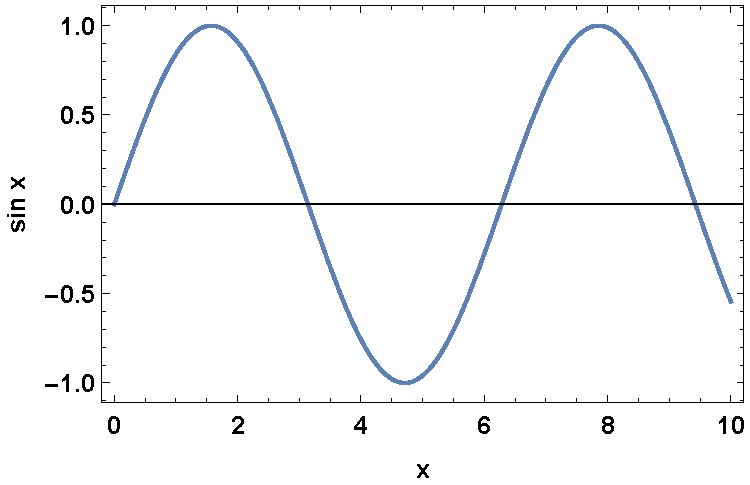
\includegraphics[width=0.5\columnwidth]{fig1.pdf}
\caption{A sine wave plotted over $[0,10]$.}
\label{fig:sinx}
\end{figure}

\section{Conclusions}

If you have any questions, email nerccs2019@gmail.com.

\section*{Acknowledgments}

Any acknowledgments, including funding information, should be described here.

\begin{thebibliography}{99}

\bibitem{nerccsinstructions} NERCCS website. http://coco.binghamton.edu/nerccs/ Accessed on August 23rd, 2018.

\end{thebibliography}

\end{document}